% Drawing 156-8/06-5 -- folder 156-8, batch 06, archive page 120 (PDF page 121).
% Transcription: une droite portant les segments $[a_1,b_1]$, $[a_2,b_2]$, $[a_3,b_3]$, $[a_n,b_n]$, marqués de croix à l'intérieur et entre eux ; le dernier segment est tracé en gras.
% Kind: intervals on a line with crosses. Method 3 (encoded, rendered from the data). Status: ok.
% Notes: A line carrying [a1,b1], [a2,b2], [a3,b3], [an,bn] (the last bold), crosses inside and between them. The line slopes slightly on the page; kept. Encoded as segment-config/1 (crosses as points of kind cross).
% Coordinates: 1 unit = 1 mm = 1/100 of the crop width (bbox in page fractions: [0.15, 0.55, 0.95, 0.59]).
% Redrawn by Claude (claude-opus-5-5), issue #73 pilot, 2026-11-07; not checked by a human; not compiled (no TeX in the session).
% Rights: reproduces part of the work -- behind RENDER_TRANSCRIPTS, never published by itself.
\documentclass[tikz,border=3pt]{standalone}
\usepackage{amsmath,amssymb}
\usetikzlibrary{patterns,arrows.meta}
\tikzset{pencil/.style={black!45}, struck/.style={black!35}, mark/.style={circle,draw,inner sep=1.3pt}, pt/.style={circle,fill,inner sep=0.9pt}, opt/.style={circle,draw,fill=white,inner sep=1.1pt}}
\begin{document}
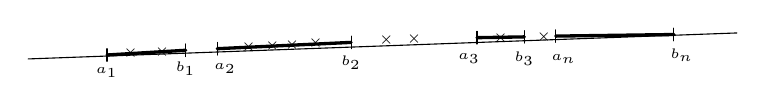
\begin{tikzpicture}[x=1mm,y=1mm,line cap=round,line join=round,font=\scriptsize]
\draw (3,-4.2) -- (93,-0.9);
\draw[very thick] (13,-3.7) -- (23,-3.1);
\draw[very thick] (27,-2.9) -- (44,-2.1);
\draw[very thick] (60,-1.5) -- (66,-1.4);
\draw[very thick] (70,-1.3) -- (85,-1.1);
\draw (13,-2.9) -- (13,-4.5);
\draw (23,-2.3) -- (23,-3.9);
\draw (27,-2.1) -- (27,-3.7);
\draw (44,-1.3) -- (44,-2.9);
\draw (60,-0.7) -- (60,-2.3);
\draw (66,-0.6) -- (66,-2.2);
\draw (70,-0.5) -- (70,-2.1);
\draw (85,-0.3) -- (85,-1.9);
\node[inner sep=1pt] at (16,-3.5) {\tiny $\times$};
\node[inner sep=1pt] at (20,-3.3) {\tiny $\times$};
\node[inner sep=1pt] at (31,-2.7) {\tiny $\times$};
\node[inner sep=1pt] at (34,-2.5) {\tiny $\times$};
\node[inner sep=1pt] at (36.5,-2.4) {\tiny $\times$};
\node[inner sep=1pt] at (39.5,-2.2) {\tiny $\times$};
\node[inner sep=1pt] at (48.5,-1.8) {\tiny $\times$};
\node[inner sep=1pt] at (52,-1.7) {\tiny $\times$};
\node[inner sep=1pt] at (63,-1.5) {\tiny $\times$};
\node[inner sep=1pt] at (68.5,-1.4) {\tiny $\times$};
\node[inner sep=1pt] at (13,-5.9) {\tiny $a_1$};
\node[inner sep=1pt] at (23,-5.4) {\tiny $b_1$};
\node[inner sep=1pt] at (28,-5.4) {\tiny $a_2$};
\node[inner sep=1pt] at (44,-4.7) {\tiny $b_2$};
\node[inner sep=1pt] at (59,-4.1) {\tiny $a_3$};
\node[inner sep=1pt] at (66,-4.2) {\tiny $b_3$};
\node[inner sep=1pt] at (71,-4.2) {\tiny $a_n$};
\node[inner sep=1pt] at (86,-3.7) {\tiny $b_n$};
\end{tikzpicture}
\end{document}
